\documentclass[11pt,a4paper]{report}
\usepackage[textwidth=37em,vmargin=30mm]{geometry}
\usepackage{calc,xunicode,amsmath,amssymb,paralist,enumitem,tabu,booktabs,datetime2,xeCJK,xeCJKfntef,listings}
\usepackage{tocloft,fancyhdr,tcolorbox,xcolor,graphicx,eso-pic,xltxtra,xelatexemoji}

\newcommand{\envyear}[0]{2025}
\newcommand{\envdatestr}[0]{2025-01-05}
\newcommand{\envfinaldir}[0]{webdb/2025/20250105/final}

\usepackage[hidelinks]{hyperref}
\hypersetup{
    colorlinks=false,
    pdfpagemode=FullScreen,
    pdftitle={Web Digest - \envdatestr}
}

\setlength{\cftbeforechapskip}{10pt}
\renewcommand{\cftchapfont}{\rmfamily\bfseries\large\raggedright}
\setlength{\cftbeforesecskip}{2pt}
\renewcommand{\cftsecfont}{\sffamily\small\raggedright}

\setdefaultleftmargin{2em}{2em}{1em}{1em}{1em}{1em}

\usepackage{xeCJK,xeCJKfntef}
\xeCJKsetup{PunctStyle=plain,RubberPunctSkip=false,CJKglue=\strut\hskip 0pt plus 0.1em minus 0.05em,CJKecglue=\strut\hskip 0.22em plus 0.2em}
\XeTeXlinebreaklocale "zh"
\XeTeXlinebreakskip = 0pt


\setmainfont{Brygada 1918}
\setromanfont{Brygada 1918}
\setsansfont{IBM Plex Sans}
\setmonofont{JetBrains Mono NL}
\setCJKmainfont{Noto Serif CJK SC}
\setCJKromanfont{Noto Serif CJK SC}
\setCJKsansfont{Noto Sans CJK SC}
\setCJKmonofont{Noto Sans CJK SC}

\setlength{\parindent}{0pt}
\setlength{\parskip}{8pt}
\linespread{1.15}

\lstset{
	basicstyle=\ttfamily\footnotesize,
	numbersep=5pt,
	backgroundcolor=\color{black!5},
	showspaces=false,
	showstringspaces=false,
	showtabs=false,
	tabsize=2,
	captionpos=b,
	breaklines=true,
	breakatwhitespace=true,
	breakautoindent=true,
	linewidth=\textwidth
}






\newcommand{\coverpic}[2]{
    % argv: itemurl, authorname
    Cover photo by #2~~(\href{#1}{#1})
}
\newcommand{\makeheader}[0]{
    \begin{titlepage}
        % \newgeometry{hmargin=15mm,tmargin=21mm,bmargin=12mm}
        \begin{center}
            
            \rmfamily\scshape
            \fontspec{BaskervilleF}
            \fontspec{Old Standard}
            \fontsize{59pt}{70pt}\selectfont
            WEB\hfill DIGEST
            
            \vfill
            % \vskip 30pt
            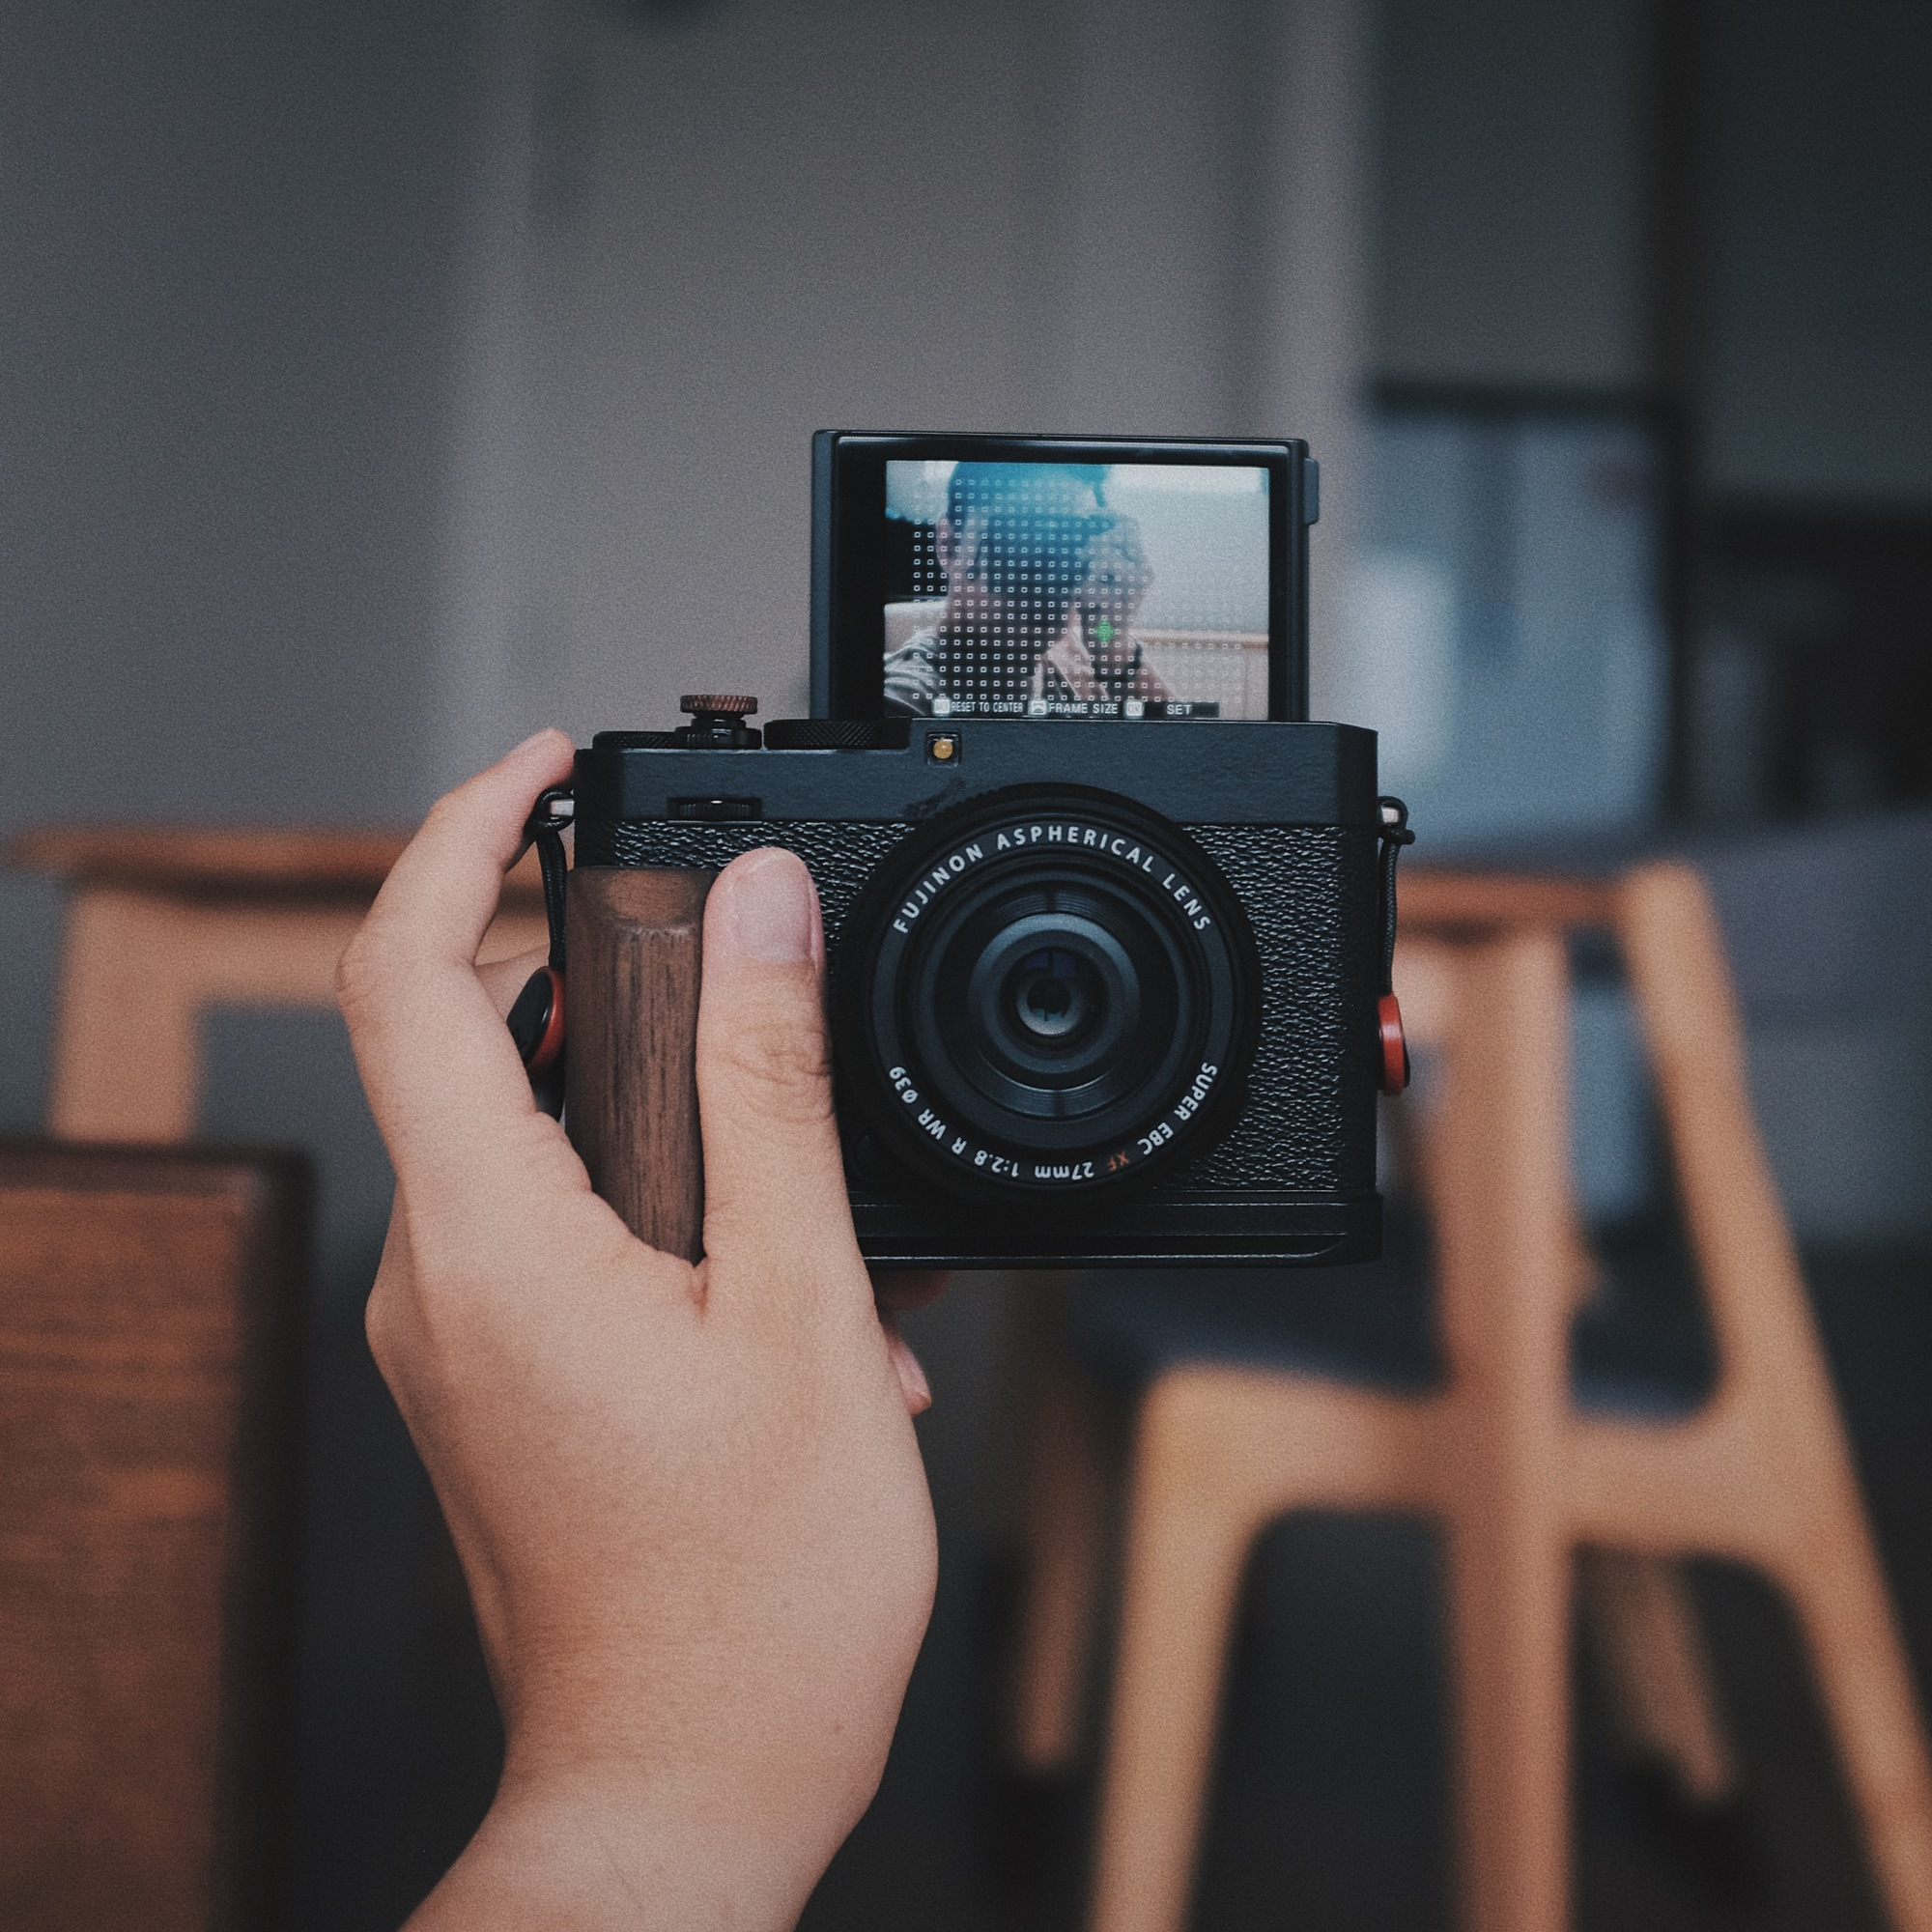
\includegraphics[width=\linewidth]{\envfinaldir/coverpic-prod.jpg}\par
            % \vskip 30pt
            \vfill

            \normalsize\rmfamily\scshape
            \copyright{} The Web Digest Project \hfill\large \envdatestr
        \end{center}
    \end{titlepage}
    % \restoregeometry
}
\newcommand{\simplehref}[1]{%
    \textcolor{blue!80!green}{\href{#1}{#1}}%
}
\renewcommand{\contentsname}{\center\Huge\sffamily\bfseries Contents\par\vskip 20pt}
\newcounter{ipartcounter}
\setcounter{ipartcounter}{0}
\newcommand{\ipart}[1]{
    % \vskip 20pt
    \clearpage
    \stepcounter{ipartcounter}
    \phantomsection
    \addcontentsline{toc}{chapter}{#1}
    % \begin{center}
    %     \Huge
    %     \sffamily\bfseries
    %     #1
    % \end{center}
    % \vskip 20pt plus 7pt
}
\newcounter{ichaptercounter}
\setcounter{ichaptercounter}{0}
\newcommand{\ichapter}[1]{
    % \vskip 20pt
    \clearpage
    \stepcounter{ichaptercounter}
    \phantomsection
    \addcontentsline{toc}{section}{\numberline{\arabic{ichaptercounter}}#1}
    \begin{center}
        \Huge
        \sffamily\bfseries
        #1
    \end{center}
    \vskip 20pt plus 7pt
}
\newcommand{\entrytitlefont}[1]{\subsection*{\raggedright\Large\sffamily\bfseries#1}}
\newcommand{\entryitemGeneric}[2]{
    % argv: title, url
    \parbox{\linewidth}{
        \entrytitlefont{#1}\par\vskip 5pt
        \footnotesize\ttfamily\mdseries
        \simplehref{#2}
    }\vskip 11pt plus 11pt minus 1pt
}
\newcommand{\entryitemGithub}[3]{
    % argv: title, url, desc
    \parbox{\linewidth}{
        \entrytitlefont{#1}\par\vskip 5pt
        \footnotesize\ttfamily\mdseries
        \simplehref{#2}\par\vskip 5pt
        \small\rmfamily\mdseries#3
    }\vskip 11pt plus 11pt minus 1pt
}
\newcommand{\entryitemAp}[3]{
    % argv: title, url, desc
    \parbox{\linewidth}{
        \entrytitlefont{#1}\par\vskip 5pt
        \footnotesize\ttfamily\mdseries
        \simplehref{#2}\par\vskip 5pt
        \small\rmfamily\mdseries#3
    }\vskip 11pt plus 11pt minus 1pt
}
\newcommand{\entryitemHackernews}[3]{
    % argv: title, hnurl, rawurl
    % \parbox{\linewidth}{
    %     \entrytitlefont{#1}\par\vskip 5pt
    %     \footnotesize\ttfamily\mdseries
    %     \simplehref{#3}\par
    %     \textcolor{black!50}{\href{#2}{#2}}
    % }\vskip 11pt plus 11pt minus 1pt
    \begin{minipage}{\linewidth}
            \entrytitlefont{#1}\par\vskip 5pt
            \footnotesize\ttfamily\mdseries
            \simplehref{#3}\par
            \textcolor{black!50}{\href{#2}{#2}}
    \end{minipage}\par\vskip 11pt plus 11pt minus 1pt
}







\begin{document}

\makeheader

\tableofcontents\clearpage




\ipart{Developers}
\ichapter{Hacker News}
\entryitemTwoLinks{US newspapers are deleting old crime stories, offering subjects a 'clean slate'}{https://news.ycombinator.com/item?id=42595307}{https://www.theguardian.com/us-news/2025/jan/04/newspaper-crime-stories}

\entryitemTwoLinks{Combining 15s interval whole-sky-camera photos to form a 4y spanning keogram}{https://news.ycombinator.com/item?id=42595190}{https://astrodon.social/@cgbassa/113770318993975063}

\entryitemTwoLinks{A mole infiltrated the highest ranks of American militias}{https://news.ycombinator.com/item?id=42594766}{https://www.propublica.org/article/ap3-oath-keepers-militia-mole}

\entryitemTwoLinks{Using LLMs and Cursor to finish side projects}{https://news.ycombinator.com/item?id=42594256}{https://zohaib.me/using-llms-and-cursor-for-finishing-projects-productivity/}

\entryitemTwoLinks{One Dog vs. the Windows 3.1 Graphics Stack}{https://news.ycombinator.com/item?id=42594024}{https://wuffs.org/blog/windows-3x-graphics}

\entryitemTwoLinks{How to draw an outline in a video game}{https://news.ycombinator.com/item?id=42593614}{https://ameye.dev/notes/rendering-outlines/}

\entryitemTwoLinks{Self driving 1993 Volvo with open pilot}{https://news.ycombinator.com/item?id=42592910}{https://practicapp.com/carbagepilot-part1/}

\entryitemTwoLinks{China is the manufacturing superpower}{https://news.ycombinator.com/item?id=42592665}{https://cepr.org/voxeu/columns/china-worlds-sole-manufacturing-superpower-line-sketch-rise}

\entryitemTwoLinks{Programming as Theory Building [pdf]}{https://news.ycombinator.com/item?id=42592543}{https://pages.cs.wisc.edu/~remzi/Naur.pdf}

\entryitemTwoLinks{Breaking Up with Long Tasks or: how I learned to group loops and wield the yield}{https://news.ycombinator.com/item?id=42592224}{https://calendar.perfplanet.com/2024/breaking-up-with-long-tasks-or-how-i-learned-to-group-loops-and-wield-the-yield/}

\entryitemTwoLinks{Do Files want to be Actors?}{https://news.ycombinator.com/item?id=42592126}{https://lewiscampbell.tech/blog/250104.html}

\entryitemTwoLinks{I'm quitting the Washington Post}{https://news.ycombinator.com/item?id=42591221}{https://anntelnaes.substack.com/p/why-im-quitting-the-washington-post}

\entryitemTwoLinks{The State of Generative Models}{https://news.ycombinator.com/item?id=42591029}{https://nrehiew.github.io/blog/2024/}

\entryitemTwoLinks{Conscious unbossing}{https://news.ycombinator.com/item?id=42590992}{https://www.robertwalters.co.uk/insights/news/blog/conscious-unbossing.html}

\entryitemTwoLinks{Meta is killing off its AI-powered Instagram and Facebook profiles}{https://news.ycombinator.com/item?id=42590981}{https://www.theguardian.com/technology/2025/jan/03/meta-ai-powered-instagram-facebook-profiles}

\entryitemTwoLinks{In Colorado, a marriage of solar energy and farming}{https://news.ycombinator.com/item?id=42590903}{https://www.ksjd.org/2024-12-31/in-colorado-a-marriage-of-solar-energy-and-farming-provides-a-model-for-a-more-sustainable-future}

\entryitemTwoLinks{A path to O1 open source}{https://news.ycombinator.com/item?id=42590322}{https://arxiv.org/abs/2412.14135}

\entryitemTwoLinks{F-Droid Fake Signer PoC}{https://news.ycombinator.com/item?id=42590307}{https://github.com/obfusk/fdroid-fakesigner-poc}

\entryitemTwoLinks{Parasitic worms 'manipulate' mantises onto asphalt roads, say researchers}{https://news.ycombinator.com/item?id=42590055}{https://mainichi.jp/english/articles/20241115/p2a/00m/0sc/009000c}

\entryitemTwoLinks{Perplexity got ads}{https://news.ycombinator.com/item?id=42589863}{https://twitter.com/damengchen/status/1875296442417607072}\ichapter{Phoronix}
\entryitemGeneric{\hskip 0pt{}Rusticl OpenCL Driver Nearing Cross-Vendor Shared Virtual Memory Support}{https://www.phoronix.com/news/Rusticl-Cross-Vendor-SVM}

\entryitemGeneric{\hskip 0pt{}GNOME Now Has Refine As An Alternative To GNOME Tweaks, Phosh 0.44 Released}{https://www.phoronix.com/news/GNOME-Starts-2025}

\entryitemGeneric{\hskip 0pt{}LLVM Had Another Exciting Year With More Than 37k Commits, 35.5 Million Lines}{https://www.phoronix.com/news/LLVM-Code-Activity-2024}

\entryitemGeneric{\hskip 0pt{}KDE Starts 2025 With Accessibility Improvements \& Better Graphics Tablet Controls}{https://www.phoronix.com/news/KDE-This-Week-Starts-2025}

\entryitemGeneric{\hskip 0pt{}Wine 10.0-rc4 Released With Another 13 Bugs Fixed}{https://www.phoronix.com/news/Wine-10.0-rc4-Released}

\entryitemGeneric{\hskip 0pt{}New Linux Patches Enhance AMD Radeon Video Encode/Decode For Older GPUs}{https://www.phoronix.com/news/Mesa-25-Better-UVD-VCE-Radeon}

\entryitemGeneric{\hskip 0pt{}Cloudflare Talks Up Multi-Path TCP But Dings Linux's Less Than Ideal Support}{https://www.phoronix.com/news/Cloudflare-MPTCP-Multi-Path-TCP}

\entryitemGeneric{\hskip 0pt{}LibreOffice 25.2 RC1 Brings Many Open-Source Office Suite Improvements}{https://www.phoronix.com/news/LibreOffice-25.2-RC1}

\entryitemGeneric{\hskip 0pt{}systemd Saw A Record Number Of Commits In 2024}{https://www.phoronix.com/news/systemd-Git-Stats-EOY-2024}


\ipart{Developers~~~~(zh-Hans)}
\ichapter{Solidot}
\entryitemGeneric{\hskip 0pt{}美国卫生局局长呼吁为酒加入致癌警告}{https://www.solidot.org/story?sid=80238}

\entryitemGeneric{\hskip 0pt{}黑客通过钓鱼攻击入侵数十个 Chrome 扩展植入后门}{https://www.solidot.org/story?sid=80237}

\entryitemGeneric{\hskip 0pt{}国补将扩大到手机、平板和智能手表等设备}{https://www.solidot.org/story?sid=80236}

\entryitemGeneric{\hskip 0pt{}Windows 10 仍然占据了最大的市场份额}{https://www.solidot.org/story?sid=80235}

\entryitemGeneric{\hskip 0pt{}2024 年挪威销售的九成汽车是纯电}{https://www.solidot.org/story?sid=80234}

\entryitemGeneric{\hskip 0pt{}美国商务部表示考虑限制或禁止中国制造的无人机}{https://www.solidot.org/story?sid=80233}

\entryitemGeneric{\hskip 0pt{}英国 2024 年可再生能源占了电力供应的 45\%}{https://www.solidot.org/story?sid=80232}

\entryitemGeneric{\hskip 0pt{}中国二氧化硫排放量过去 15 年减少了三分之二以上}{https://www.solidot.org/story?sid=80231}

\entryitemGeneric{\hskip 0pt{}蝙蝠一夜之间能飞行近 400 公里}{https://www.solidot.org/story?sid=80230}

\entryitemGeneric{\hskip 0pt{}苹果和 Google 在印度的应用商店下架了多款 VPN 应用}{https://www.solidot.org/story?sid=80229}

\entryitemGeneric{\hskip 0pt{}巨鲸能活得 130 岁以上}{https://www.solidot.org/story?sid=80228}

\entryitemGeneric{\hskip 0pt{}全球生育率下滑和宏观经济发展}{https://www.solidot.org/story?sid=80227}

\entryitemGeneric{\hskip 0pt{}特斯拉全球销量首次下降}{https://www.solidot.org/story?sid=80226}

\entryitemGeneric{\hskip 0pt{}埃博拉病毒可能通过触摸皮肤直接传播}{https://www.solidot.org/story?sid=80225}

\entryitemGeneric{\hskip 0pt{}龙芯开发者向内核递交 32 位 LoongArch CPU 架构支持}{https://www.solidot.org/story?sid=80224}

\entryitemGeneric{\hskip 0pt{}气候变化导致加拿大野火加剧}{https://www.solidot.org/story?sid=80223}

\entryitemGeneric{\hskip 0pt{}普京命令俄罗斯加强与中国在 AI 上的合作}{https://www.solidot.org/story?sid=80222}

\entryitemGeneric{\hskip 0pt{}无聊的城市建筑不利于你的健康}{https://www.solidot.org/story?sid=80221}

\entryitemGeneric{\hskip 0pt{}人体组织中的微塑料与特定疾病相关}{https://www.solidot.org/story?sid=80220}

\entryitemGeneric{\hskip 0pt{}小米修改了引导程序解锁政策}{https://www.solidot.org/story?sid=80219}\ichapter{V2EX}
\entryitemGeneric{\hskip 0pt{}[问与答] 这几年太多的财富是 it 届爆发的,请问 v2 各位 it 届精英,你们平时都听什么播客?}{https://www.v2ex.com/t/1102597}

\entryitemGeneric{\hskip 0pt{}[Linux] wakeup over wifi 有成功的同学吗?}{https://www.v2ex.com/t/1102595}

\entryitemGeneric{\hskip 0pt{}[互联网] tailscale 打洞成功,但是速度远低于实际带宽}{https://www.v2ex.com/t/1102594}

\entryitemGeneric{\hskip 0pt{}[问与答] 工业品过剩的时代,人类将如何生存}{https://www.v2ex.com/t/1102593}

\entryitemGeneric{\hskip 0pt{}[程序员] XXL-RPC v1.8.1 | RPC 服务框架}{https://www.v2ex.com/t/1102592}

\entryitemGeneric{\hskip 0pt{}[推广] 荷兰月付 1.44 欧, 2c/1G/50G, 10G 口无限流量机器}{https://www.v2ex.com/t/1102590}

\entryitemGeneric{\hskip 0pt{}[Surge] iOS Surge 求助}{https://www.v2ex.com/t/1102589}

\entryitemGeneric{\hskip 0pt{}[程序员] 内测第 10 天,我们成功处理了第 100 万条模型请求}{https://www.v2ex.com/t/1102588}

\entryitemGeneric{\hskip 0pt{}[VPS] 130 出一台 cc 年付 25 刀的, 2c2g100g 机器}{https://www.v2ex.com/t/1102587}

\entryitemGeneric{\hskip 0pt{}[宽带症候群] 想找一个 ping 和 traceroute 的面板}{https://www.v2ex.com/t/1102586}

\entryitemGeneric{\hskip 0pt{}[问与答] 求推荐个域名邮箱,以及我用过的域名邮箱体验}{https://www.v2ex.com/t/1102585}

\entryitemGeneric{\hskip 0pt{}[问与答] 有没有只有搜索和收藏夹功能的小红书版本(逃离信息流)}{https://www.v2ex.com/t/1102583}

\entryitemGeneric{\hskip 0pt{}[酷工作] 诚聘一名 web3 运营指导老师}{https://www.v2ex.com/t/1102582}

\entryitemGeneric{\hskip 0pt{}[程序员] Java 工资}{https://www.v2ex.com/t/1102581}

\entryitemGeneric{\hskip 0pt{}[问与答] 买的内存条只能兼容一台电脑,留还是退了?}{https://www.v2ex.com/t/1102580}

\entryitemGeneric{\hskip 0pt{}[问与答] AP 面板无线测速跑不满网速,正常吗}{https://www.v2ex.com/t/1102579}

\entryitemGeneric{\hskip 0pt{}[Google] Google 翻译怎么还不上 AI}{https://www.v2ex.com/t/1102577}

\entryitemGeneric{\hskip 0pt{}[问与答] 电报上有啥前端交流群嘛?}{https://www.v2ex.com/t/1102575}

\entryitemGeneric{\hskip 0pt{}[问与答] Parsec 在多 ip 可访问 host 的情况下能指定 ip 吗?}{https://www.v2ex.com/t/1102572}

\entryitemGeneric{\hskip 0pt{}[微信] 怎么把我的用户加到一个微信群里呢}{https://www.v2ex.com/t/1102571}

\entryitemGeneric{\hskip 0pt{}[问与答] 求问群晖 Nas 家庭影院方案,主要适配苹果全家桶就好}{https://www.v2ex.com/t/1102570}

\entryitemGeneric{\hskip 0pt{}[VPS] [限时活动] 搬瓦工新出的机器,三网 CN2 线路较好 2.5G 带宽}{https://www.v2ex.com/t/1102569}

\entryitemGeneric{\hskip 0pt{}[随想] 2025 年,我想,跳出这个怪圈吧}{https://www.v2ex.com/t/1102568}

\entryitemGeneric{\hskip 0pt{}[程序员] 你真的会看下属写的年终总结吗}{https://www.v2ex.com/t/1102567}

\entryitemGeneric{\hskip 0pt{}[Neovim] go-impl.nvim - 一个基于 impl 的 Go 接口实现插件}{https://www.v2ex.com/t/1102566}

\entryitemGeneric{\hskip 0pt{}[推广] 非常稳定的 ai-api,支持 chatgpt 、claude 、gemini 、mj 、sd 、flux 、suno 、luma 等}{https://www.v2ex.com/t/1102565}

\entryitemGeneric{\hskip 0pt{}[Apple] 求个美区 infuse 的车!}{https://www.v2ex.com/t/1102562}

\entryitemGeneric{\hskip 0pt{}[问与答] 关于跨境电商中的侵权问题}{https://www.v2ex.com/t/1102561}

\entryitemGeneric{\hskip 0pt{}[上海] 芯启源股权被冻结原因有网友知道吗?}{https://www.v2ex.com/t/1102560}

\entryitemGeneric{\hskip 0pt{}[宽带症候群] 无线网络抽风的原因是?}{https://www.v2ex.com/t/1102558}

\entryitemGeneric{\hskip 0pt{}[推广] 搬瓦工: POWERBOX 来袭,三网 CN2GIA 线路+1.5T 大流量,终于不用邀请码了}{https://www.v2ex.com/t/1102557}

\entryitemGeneric{\hskip 0pt{}[宽带症候群] 关于联通宽带晚间限速导致跨网访问拉垮}{https://www.v2ex.com/t/1102555}

\entryitemGeneric{\hskip 0pt{}[分享创造] [🎁抽奖 3 永久 5 年度] 狂肝一月重构轻翻相册,照片整理新体验, 25 年又有额度了}{https://www.v2ex.com/t/1102554}

\entryitemGeneric{\hskip 0pt{}[酷工作] [社招] 知名 AI 公司 LLM/多模态/aigc 算法/训练/推理/后端/移动}{https://www.v2ex.com/t/1102553}

\entryitemGeneric{\hskip 0pt{}[投资] 清仓 A 股了,三年,净亏损 2.6w}{https://www.v2ex.com/t/1102552}

\entryitemGeneric{\hskip 0pt{}[宽带症候群] 有了解光猫接 sip 座机吗,我通话长就会断线}{https://www.v2ex.com/t/1102550}

\entryitemGeneric{\hskip 0pt{}[问与答] 各位 V2er,已经 2025 年了,在 iPad 上查看外文的 PDF,快速查询英文单词翻译的姿势是什么?}{https://www.v2ex.com/t/1102549}

\entryitemGeneric{\hskip 0pt{}[推广] [送码]大晚上没事儿干又来搞事情了 -- DS Cloud 送码}{https://www.v2ex.com/t/1102548}

\entryitemGeneric{\hskip 0pt{}[问与答] 现阶段,语言大模型的输入输出对人类程序员来说是黑箱吗,有多少机制是已经明确了的?}{https://www.v2ex.com/t/1102547}

\entryitemGeneric{\hskip 0pt{}[问与答] 新手提问 Gemini 会不会用超}{https://www.v2ex.com/t/1102543}

\entryitemGeneric{\hskip 0pt{}[分享发现] 读《圣经》出埃及记 这段惊呆了,这是约 3500 年前的事}{https://www.v2ex.com/t/1102542}

\entryitemGeneric{\hskip 0pt{}[Apple] M2 尚能饭否}{https://www.v2ex.com/t/1102540}

\entryitemGeneric{\hskip 0pt{}[macOS] 有没有可以监控异常进程的方法}{https://www.v2ex.com/t/1102535}

\entryitemGeneric{\hskip 0pt{}[Linux] 大家有遇到过 Linux 电脑睡眠之后经常自己关机了么}{https://www.v2ex.com/t/1102534}

\entryitemGeneric{\hskip 0pt{}[Linux] 记一次 ZFS 存储池恢复实战}{https://www.v2ex.com/t/1102533}

\entryitemGeneric{\hskip 0pt{}[问与答] 炸裂}{https://www.v2ex.com/t/1102531}

\entryitemGeneric{\hskip 0pt{}[程序员] 关于今天给前端返回数据的结构的争论}{https://www.v2ex.com/t/1102528}

\entryitemGeneric{\hskip 0pt{}[阅读] 微信读书有一丢丢离谱}{https://www.v2ex.com/t/1102526}

\entryitemGeneric{\hskip 0pt{}[AirPods] 戴 AirPods Pro 的时候如果有人打电话过来,音量会突然变成最大值,震耳欲聋,如何解决}{https://www.v2ex.com/t/1102525}

\entryitemGeneric{\hskip 0pt{}[云修电脑] 服务器装 Ubuntu22.04 死机}{https://www.v2ex.com/t/1102524}


\ipart{Generic News}
\ichapter{联合早报}
\entryitemWithDescription{沈泽玮:台湾冲突阻遏法案只叫不咬?}{https://www.zaobao.com/news/china/story20240918-4758889}{美国众议院9月9日开启了长达一星期的``中国周'',共通过25项主要涉华法案。(法新社) 美国众议院在当地时间9月9日开启了长达一星期的``中国周'',在美国总统和国会选举举行之前,密集表决数十项与中国有关的法案,共通过25项主要涉华法案……}

\entryitemWithDescription{欧盟电动车关税投票倒计时 中国在分歧中寻支持}{https://www.zaobao.com/news/china/story20240917-4758953}{欧盟27个成员国将于9月25日就是否继续对进口自中国的电动汽车额外征税进行最后表决。图为上海港等待装运出口的电动汽车。(彭博社) 欧盟对中国电动汽车加征关税的投票进入倒计时,正在欧洲访问的中国商务部部长王文涛与欧盟多国政府高层就此进行协商,试图在立场分歧的成员国中争取到更多支持。 受访学者研判,欧盟对中国电动汽车加征关税不可避免,但具体的加税方式和幅度仍有一定弹性,这是王文涛此行与各国谈判的重点……}

\entryitemWithDescription{港府今年将举办逾400项国庆活动}{https://www.zaobao.com/news/china/story20240917-4759341}{再过十多天就是中国国庆75周年,香港天星小轮展示``国庆75周年''\,``三天免费搭小轮''等标语迎国庆。(中新社) 再过十多天就是中国国庆75周年,香港特区政府今年将举办逾400项庆祝活动,希望通过一连串活动庆祝国庆,并且弘扬爱国主义教育及刺激消费。 港府星期二(9月17日)召开记者会,介绍各项庆祝国庆活动和特别优惠,涉及出行及吃喝玩乐等领域……}

\entryitemWithDescription{美空军部长:中国大陆军演精密化 为入侵封锁台湾做准备}{https://www.zaobao.com/news/china/story20240917-4759407}{美国空军部长肯德尔星期一(9月16日)在空军暨太空军协会的一场大会上致辞,提到中国对印太地区日益增长的威胁。(取自美国国防部网站) (华盛顿综合讯)美国空军部长肯德尔指,中国大陆军演的规模越来越大,也更加精密化,这是在专门为入侵、封锁台湾做准备。他也称,中国对印太地区的威胁现在已存在……}

\entryitemWithDescription{批准潜在对台备件军售案后 美派巡逻机过航台海}{https://www.zaobao.com/news/china/story20240917-4758770}{台军士兵8月26日在屏东县枋山训练场进行实弹演习时,从M1167 TOW运载车上发射一枚美制TOW-2A线导反坦克导弹。(路透社) (华盛顿/台北/北京综合讯)在批准潜在对台备件军售案之后,美国派遣反潜巡逻机过航台湾海峡,中国人民解放军东部战区则组织战机跟监美机,并誓言``坚决捍卫国家主权''……}

\entryitemWithDescription{李家超:若香港驻美经贸办被关 受害的是美企}{https://www.zaobao.com/news/china/story20240917-4758797}{香港特首李家超星期一(9月17日)警告,如果美国通过法案,导致香港驻美经贸办关闭,受害的是美国企业。图为李家超9月11日在``一带一路''高峰论坛上致辞。(彭博社) (香港综合讯)香港特首李家超警告,如果美国通过法案,导致香港驻美经贸办关闭,受害的是美国企业。 美国众议院上周通过《香港经济贸易办事处认证法案》,如果参议院也表决通过并交由总统签署成法,香港三个驻美国的经贸办可能将被强制关闭……}

\entryitemWithDescription{美国指中国航空工业集团员工企图实施黑客攻击}{https://www.zaobao.com/news/china/story20240917-4757988}{(华盛顿综合讯)中国航空航天巨头中国航空工业集团一名员工被指试图对美国宇航局、美国军方和其他目标展开黑客攻击。 据彭博社报道,美国检察官布坎南星期一(9月16日)在起诉书中,指控中国航空工业集团39岁的工程师吴宋(音译,Song Wu)企图从美国宇航局、空军、陆军和海军,以及联邦航空管理局取得电脑软件和源代码……}

\entryitemWithDescription{【东谈西论】恒大账务造假 普华永道是共犯还是被拖累?}{https://www.zaobao.com/news/china/story20240917-4756452}{因涉及恒大地产审计项目的违法行为,普华永道中国9月13日被中国财政部和证监会处以4.41亿人民币罚款并被令停业六个月, 广州分所被撤销……}

\entryitemWithDescription{戴庆成:香港输入人才计划大检阅}{https://www.zaobao.com/news/china/story20240917-4744978}{香港于2022年底推出高端人才通行证计划。(法新社) 2019年香港反修例风波过后,数以十万计港人移居海外,令香港出现人才荒。港府为了解决这个问题,在过去几年积极引入``新血'',当中以高才通计划最受瞩目,社会上也不时热议其成效。 高才通全称为高端人才通行证计划,于2022年底推出,申请人年收入须达到250万港元(约42万新元)以上,或本科毕业于全球百强大学并满足一定工作年限等……}

\entryitemWithDescription{中美希望稳定双边关系 中小国家可​​​搭建桥梁}{https://www.zaobao.com/news/china/story20240917-4745091}{中美元首去年11月在旧金山会晤后,双方都希望稳定两国关系,我国巡回大使陈庆珠认为,如果中美两国都认为走向战争不符合它们的利益,那么中小国家就可以做点什么,为双方搭建桥梁。 陈庆珠星期一(9月16日)在李光耀公共政策学院的一场研讨会上说,中国与西方的关系面对诸多困难,有中国智库表示,希望新加坡能协助在中美之间建立更多对话,``因为新加坡受美国信任,也在中国有渠道''……}

\entryitemWithDescription{陈庆珠:世界经历了三次``中国冲击'' 中美的主导力之争将继续}{https://www.zaobao.com/news/china/story20240917-4744996}{李光耀公共政策学院``思想之节庆''的一场研讨会,讨论``历史终结时的中国冲击''。左起是我国巡回大使陈庆珠、通商中国主席李奕贤、李光耀公共政策学院国际关系助理教授何莉菁、李光耀公共政策学院院长柯成兴……}

\entryitemWithDescription{上海遭遇75年来最强台风 扰乱民众中秋假期出行}{https://www.zaobao.com/news/china/story20240916-4745224}{台风贝碧嘉星期一(9月16日)登陆上海,维护人员星期一下午在衡山路上处理倒伏的树木。 (新华社) 台风造成上海上万株数目倒伏或折断。图为一棵倒下的大树砸坏一旁的建筑。(法新社) 台风贝碧嘉登陆上海后,黄浦江苏州河口潮位上涨,乌云密布。(中新社) 中国上海市星期一(9月16日)遭遇75年来最强台风``贝碧嘉''登陆,也是上海有记录以来首次有强台风侵袭……}

\entryitemWithDescription{陆男频长驱偷渡台湾在测试边防实力?}{https://www.zaobao.com/news/china/story20240916-4745161}{中国大陆一名王姓男子在中秋节前夕,乘橡皮艇从浙江宁波抵达台湾新北市林口,主动打电话投案,海巡署人员前去接他上岸。(自由時報) 中国大陆一名王姓男子划橡皮艇于上星期六清晨偷渡到台湾,隔天被新北市地方法院裁定羁押禁见。这是6月以来第二起大陆人士偷渡至台湾,此间专家质疑是否为海防破口,并怀疑对岸是否在测试台湾的边防实力……}

\entryitemWithDescription{中美时隔八月举行国防部工作会晤}{https://www.zaobao.com/news/china/story20240916-4745025}{(北京/华盛顿综合讯)中美双方上周末举行国防部工作会晤;美国官员称,美国积极进行美中两军外交活动,不代表美国对有关中国议题的处理方式发生任何改变。 据中国国防部星期天(15日)晚上通报,北京香山论坛结束后,第18次中美国防部工作会晤上星期六至星期天(9月14日至15日)在北京举行……}

\entryitemWithDescription{中国高校今年拟增足球运动本科专业}{https://www.zaobao.com/news/china/story20240916-4744925}{(北京综合讯)为了培养足球专业人才,中国大专学府今年度拟新增足球运动本科专业,以具体落实中国足球改革。 综合人民网和《南方都市报》报道,中国教育部上星期五(9月13日)发布《2024年度普通高等学校本科专业申报材料公示》。根据公示统计,今年度拟新增专业535个,涉及353所高校,其中39所高校新增足球运动专业……}

\entryitemWithDescription{香港23条首案 港男因穿``光时''上衣被定罪}{https://www.zaobao.com/news/china/story20240916-4743439}{(香港综合讯)香港一名无业男子,今年6月因穿印有2019年反修例抗争口号的上衣而被捕。他星期一承认违反煽动意图罪,成为在《维护国家安全条例》(即《香港基本法》第23条)下被定罪的第一人。 综合港媒《星岛日报》和路透社报道,27岁无业男子诸启邦今年6月12日在石门港铁站附近,未能出示身份证供查阅被警方拘捕……}

\entryitemWithDescription{美国务院:中国释放被关押近20年美籍牧师}{https://www.zaobao.com/news/china/story20240916-4744614}{(华盛顿综合电)中国释放被关押近20年的美国籍牧师,显示北京在中美关系的关键时刻展现善意。 综合彭博社、法新社和路透社报道,美国国务院发言人星期天(9月15日)说:``我们欢迎林大卫(音译,David Lin)从中华人民共和国的监狱获释。他已回返美国,这是他近20年来首次与家人见面。'' 林大卫的女儿艾丽斯告诉美国政治新闻网Politico,她的父亲将抵达得克萨斯州的圣安东尼奥……}

\entryitemWithDescription{中国驻泰使馆:近期并未向湄公河下游泄洪}{https://www.zaobao.com/news/china/story20240916-4743917}{(北京讯)泰国西北部的湄公河因洪水泛滥而决堤,中国否认这是中方泄洪所致,并称近来已持续减少云南景洪水电站的出库流量,以助下游地区抗洪。 中国驻泰国大使馆星期日(9月15日)深夜在官方微信公众号发文说,当天又有媒体报道称中国正在向湄公河泄洪,经向中国主管部门核实,使馆再次澄清,为帮助下游地区应对洪灾,中方近来持续稳定和减少景洪水电站出库流量,不可能对下游地区抗洪救灾形成压力……}

\entryitemWithDescription{加入美国储存可靠度评估计划 台湾军方编列预算采购三类型导弹}{https://www.zaobao.com/news/china/story20240916-4743826}{(台北讯)据台媒报道,台湾军方持续向美国采购可简易操作的导弹,预计在2024年、2031年以前获得400枚``标枪''反装甲导弹、2485枚``刺针''人携式防空导弹……}

\entryitemWithDescription{韩咏红:中美分头追逐全球南方}{https://www.zaobao.com/news/china/story20240916-4730719}{9月5日,中国外长王毅(中)同中非合作论坛非方现任共同主席国塞内加尔外长法勒(左)、下任共同主席国刚果外长加科索(右),在北京共同会见中外记者并答问。(路透社) 进入气候宜人的9月,中国接连举行了两场受瞩目的国际会议,一是聚集非洲53国国家元首与政要的中非合作论坛,接着是周末刚闭幕的北京香山论坛。 两场活动的参与者不同,规模也有很大差距……}

\entryitemWithDescription{菲律宾船只撤离中菲争议海域后 将再派船接替}{https://www.zaobao.com/news/china/story20240915-4730494}{这张在9月15日拍摄,并由菲律宾海岸警卫队提供的照片显示,菲律宾海岸警卫队船马格巴努亚号抵达了菲国巴拉望岛的一个港口。菲律宾早前以发现填海活动为由,今年4月派出马格巴努亚号前往萨比纳礁。(法新社/菲律宾海岸警卫队) 菲律宾国家海事委员会星期天(9月15日)发声明称,该国海岸警卫队一艘巡逻舰已离开萨比纳礁争议海域……}

\entryitemWithDescription{台风贝碧嘉直击中国华东 多趟本地与沪杭间航班取消}{https://www.zaobao.com/news/china/story20240915-4730611}{9月15日在上海外滩滨江步道上,一名外籍游客的雨伞被大风吹起。台风贝碧嘉的中心当天下午5时位于上海市东偏南方大约435公里的东海海面上,中心附近最大风力有13级。(中新社) (上海/新加坡综合讯)台风贝碧嘉预计将为中国华东沿海地区带来狂风暴雨,多趟往返新加坡与上海和杭州的航班取消……}






\clearpage
\leavevmode\vfill
\footnotesize

Copyright \copyright{} 2023-2025 Neruthes and other contributors.

This document is published with CC BY-NC-ND 4.0 license.

The entries listed in this newsletter may be copyrighted by their respective creators.

This newsletter is generated by the Web Digest project.

The newsletters are also delivered via Telegram channel \CJKunderline{\href{https://t.me/webdigestchannel}{https://t.me/webdigestchannel}}.\\
RSS feed is available at \CJKunderline{\href{https://webdigest.pages.dev/rss.xml}{https://webdigest.pages.dev/rss.xml}}.

This newsletter is available in PDF at
\CJKunderline{\href{https://webdigest.pages.dev/}{https://webdigest.pages.dev/}}.

The source code being used to generate this newsletter is available at\\
\CJKunderline{\href{https://github.com/neruthes/webdigest}{https://github.com/neruthes/webdigest}}.

This newsletter is also available in
\CJKunderline{\href{http://webdigest.pages.dev/readhtml/\envyear/WebDigest-20250105.html}{HTML}} and
\CJKunderline{\href{https://github.com/neruthes/webdigest/blob/master/markdown/\envyear/WebDigest-20250105.md}{Markdown}}.


\coverpic{}{}


\end{document}
